\documentclass[12pt, titlepage]{article}
\usepackage[shortlabels]{enumitem}
\usepackage{comment}
\usepackage{booktabs}
\usepackage{tabularx}
\usepackage{hyperref}
\usepackage{float}
\usepackage{soul}
\usepackage{changepage}
\usepackage{graphicx}
\setstcolor{red}
\hypersetup{
    colorlinks,
    citecolor=black,
    filecolor=black,
    linkcolor=black,
    urlcolor=blue
}
\usepackage[dvipsnames]{xcolor}
\usepackage[round]{natbib}

%% Comments

\usepackage{color}

\newif\ifcomments\commentstrue %displays comments
%\newif\ifcomments\commentsfalse %so that comments do not display

\ifcomments
\newcommand{\authornote}[3]{\textcolor{#1}{[#3 ---#2]}}
\newcommand{\todo}[1]{\textcolor{red}{[TODO: #1]}}
\else
\newcommand{\authornote}[3]{}
\newcommand{\todo}[1]{}
\fi

\newcommand{\wss}[1]{\authornote{blue}{SS}{#1}} 
\newcommand{\plt}[1]{\authornote{magenta}{TPLT}{#1}} %For explanation of the template
\newcommand{\an}[1]{\authornote{cyan}{Author}{#1}}

%% Common Parts

\newcommand{\progname}{ProgName} % PUT YOUR PROGRAM NAME HERE
\newcommand{\authname}{Team \#, Team Name
\\ Student 1 name
\\ Student 2 name
\\ Student 3 name
\\ Student 4 name} % AUTHOR NAMES                  

\usepackage{hyperref}
    \hypersetup{colorlinks=true, linkcolor=blue, citecolor=blue, filecolor=blue,
                urlcolor=blue, unicode=false}
    \urlstyle{same}
                                


\setcitestyle{numbers}

\title{SE 4G06: Software Requirements Specification\\\textit{Measuring Microstructure Changes During Thermal Treatment }}

\author{\authname}

\date{}

\begin{document}

\maketitle

\pagenumbering{roman}
\tableofcontents
\listoftables
\listoffigures

\begin{table}[H]
\caption{\bf Revision History}
\begin{tabularx}{\textwidth}{p{2.5cm}p{2.5cm}X}
\toprule {\bf Date} & {\bf Developer} & {\bf Notes/Changes}\\
\midrule
Sept 25, 2022 & Edwin Do & Revision 0 - Initial commit\\
Oct 5, 2022 & Edwin Do & Adopt Volere template + Add content \\
Oct 5, 2022 & Timothy Chen & Added to Non-Functional Requirements\\
Oct 5, 2022 & Abdul Nour Seddiki & Added to Relevant Facts and Assumptions\\
Oct 5, 2022 & Abdul Nour Seddiki & Added to Waiting Room\\
Oct 5, 2022 & Timothy Chen & Added to Reflection\\
Oct 5, 2022 & Joseph Braun & Add functional Requirements \\ 
Oct 5, 2022 & Abdul Nour Seddiki & Added to Reflections\\
Oct 5, 2022 & Edwin Do & Add reflection + small fixes \\
Oct 6, 2022 & Edwin Do & Add missing tasks, ideas for solution, and open issues \\
Oct 31, 2022 & Edwin Do & Update with the use of Visual Studio\\
Mar 8, 2023 & Abdul Nour Seddiki & Added two functional requirements\\
\bottomrule
\end{tabularx}
\end{table}

\newpage

\pagenumbering{arabic}

\noindent This document describes the software requirements for the capstone project of measuring microstructure changes of samples during thermal treatment. The template for the Software Requirements Specification (SRS) is a subset of the Volere
template.


\section{Project Drivers}

\subsection{The Purpose of the Project}
The purpose of this project is to assist the Department of Materials Engineering in measuring the changes to a material's microstructure during thermal treatment. 
By doing so, the resistivity of the sample can be measured at different thermal levels. The goal is to be able to collect the data at necessary sampling rate and 
incorporate the use of Windows GUI. 

\subsection{The Stakeholders}

\subsubsection{Developers}
The Developers will be responsible for the design, development, and documentation throughout. They will be utilizing the existing lab equipment, computer for the duration of this project.
Developers will also use the feedback from the client to deliver the final product. 

\subsubsection{The Client}
The Client for this project is the Department of Materials Engineering and the Computing and Software Department at McMaster University. More specifically, Dr. Zurob, Dr. Smith and TAs of 4G06 who will be the ones to evaluate, review and provide feedback on the project throughout the development process.

\subsubsection{The Customers}
The Customers for this project are anyone who will be conducting research or require data that measures the microstructural changes of materials under various thermal treatment.   

\subsubsection{Other Stakeholders}
This project has no other stakeholders.

\subsection{Mandated Constraints}

\subsubsection{Solution Constraints}

Description: The GUI will run on Windows operating system\\ 
Rationale: The application is a Desktop application. The lab computer that has the capability to connect to other required lab equipment currently runs on Windows.\\
Fit Criterion: Users can successfully install and open the application on a supported Windows operating system. \\

\noindent Description: The sampling rate of the equipment to the GUI will be at least 100 times per second\\ 
Rationale: According to Dr.Zurob, this is the minimum sampling rate needed to see any meaningful data\\
Fit Criterion: The equipment samples the data at 100 times per second and the GUI accurately reflects the measurements  \\

\subsubsection{Off-the-shelf Software}
No off-the-shelf software is required for this project. 

\subsubsection{Anticipated Workplace Environment}
The software and equipment will be designed for the expected environment of a lab. The reason is that the lab equipment and computer is needed for the software to run successfully and
should not be easily accessible outside of campus. 

\subsubsection{Schedule Constraints}
% Add other deadlines
The deadline for the final product is the March 20 2023. There will be other milestones during the development process that must be accomplished throughout. 
This will be outlined in our Github milestones.


\subsubsection{Budget Constraints}
% Double check this
At this point, there is an estimated budget of \$1000. This may change as the team determines what additional equipment is needed to work with the lab equipment.

\subsection{Naming Conventions and Terminology}

\begin{itemize}
    \item \textbf{C\#}: Scripting language used to create and control dynamic content.
    \item \textbf{Visual Studio}: Standard markup language for creating web pages.
    \item \textbf{UWP}: Style sheet language for structuring and styling HTML web page.
    \item \textbf{Windows}: A popular operating system used by many users.
    \item \textbf{Product/Software/Application}: Refers to the final deliverable of this capstone project.
    \item \textbf{User}: The person who will be interacting/ using the application.
\end{itemize}

\subsection{Relevant Facts and Assumptions}
\subsubsection{Facts}
The client and control computer is using Windows XP operating system that is questionably upgradable and it is worth mentioning that Windows XP is currently unsupported. The equipment for power supply and measurement tools are outdated and require special connection media, both physical connections and drivers, to communicate with the computer. There exists an application with a similar purpose and function to our project’s on the computer, which does not fulfill the goals of the user anymore, and the source code for that application is not provided.\\

\noindent Resistivity of a sample material is calculated by the following equation. Where $\rho$ is the resistivity, R is the resistance, A is the cross-sectional area, and L is the length of the sample:
$ \rho = \frac{RA}{L} $
% Include a couple sentences about the background and maybe an equation describing how the conductivity is calculated.

\subsubsection{Assumptions}
Statement: It is assumed that materials will have microstructural changes when they undergo heat treatment. 
Effect: In case this assumption is false, our product will display no output. \\

\noindent Statement: Another assumption is that these microstructural changes will result in changes in resistivity of the materials treated. 
Effect: If this assumption is false, the product will be rendered unsuitable for the task as the main function of it is to measure changes in resistivity.\\

\noindent Statement: According to the project timeline, it is assumed that a proof of concept will be ready by November 14th, a first functional design will be ready by February 6th, and a final revision will be demoed by March 31st.
Effect: These dates are made to observe progress of the project. In case the final demo is not met, the project will have been incomplete, since that will be the end of term for the developers.
% Include a couple sentences about any assumptions that we have

\subsubsection{User Characteristics}
An assumption made about this project is that the users will have the necessary knowledge to safely operate the necessary lab equipment. This is required to collect the data and display it on the GUI. 
The user is also assumed to have general working knowledge of how to install and open a windows application, as well as the use of a mouse and keyboard input. Another assumption is that the user is literate in English.

\section{Functional Requirements}
\subsection{The Scope of the Work and the Product}

The hardware for this project is provided by the Department of Materials Engineering through the project supervisor, Dr. Zurob. A Windows computer, current source, and nanovoltmeter have already been included. A fourth hardware device, for measuring the temperature of the sample material, will also be provided or else a new device shall be purchased for this purpose. The product will be a Window's based GUI application which can set the data acquisition rate (sample rate), connect to the hardware devices, acquire the output data, and calculate the conductivity of the sample material in real time. The application should also be able to be accessed remotely to check on the progress of ongoing experiments. \\

\subsubsection{The Context of the Work}
% Electron - JS, HTML , CSS
% CI/CD - Build
% Devs may require the use of other libraries to speed up the dev process
\begin{figure}[H]
\centerline{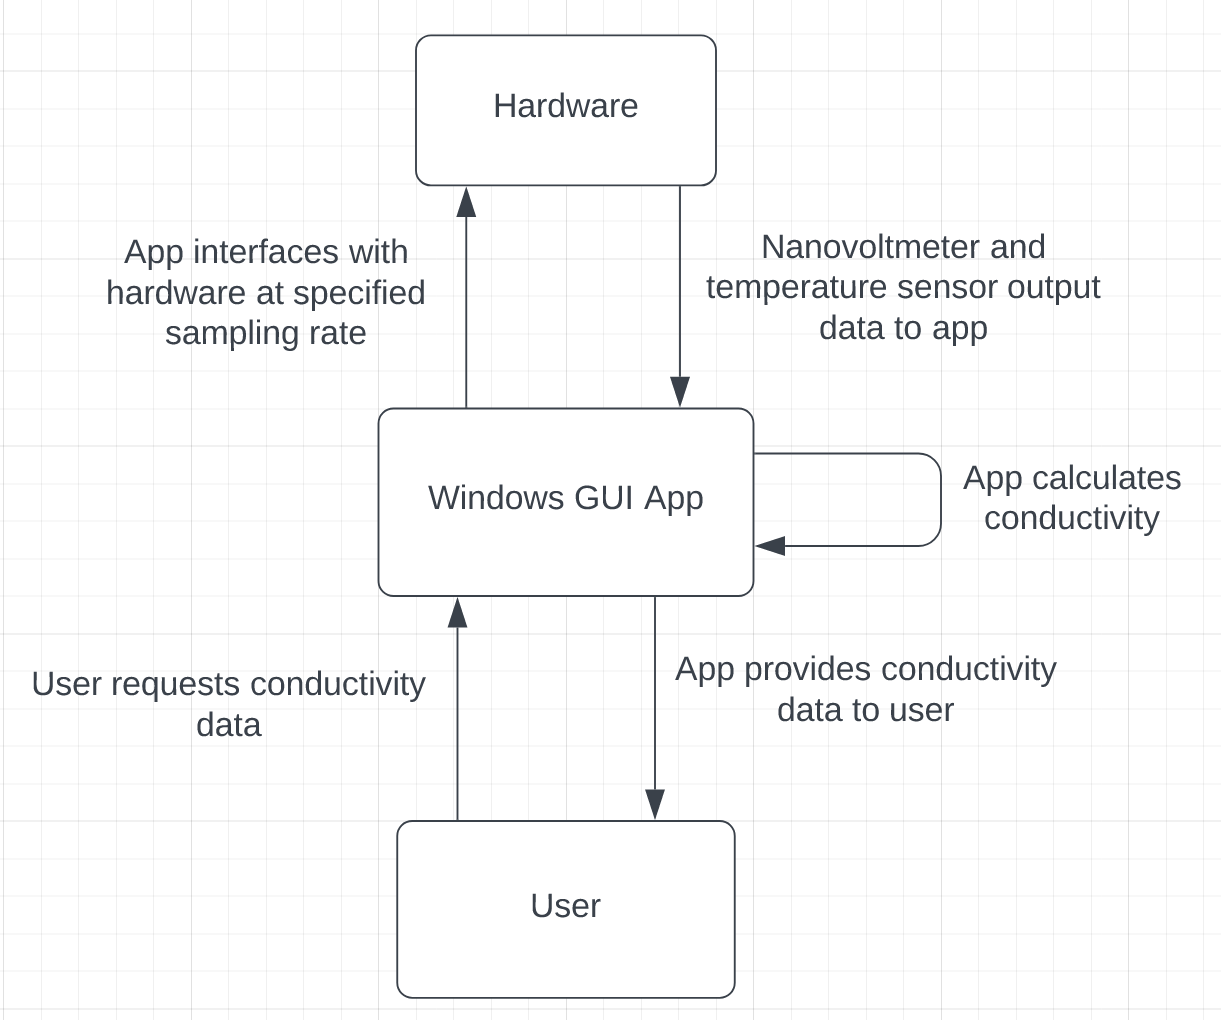
\includegraphics[scale=0.8]{ContextDiagram.PNG}}
\caption{Basic context diagram (subject to change as project progresses)}
\label{fig}
\end{figure}

\subsubsection{Work Partitioning}

\begin{table}[H]
	\centering
	\caption{Work Partitioning}
	\label{my-label}
	\begin{tabular}{|c|c|c|c|}
		\hline
		\textbf{Event \#} & \textbf{Event Name} & \textbf{Input} & \textbf{Output}     \\ \hline
		1 & \begin{tabular}{@{}c@{}}User requests\\conductivity data\end{tabular} & 
            \begin{tabular}{@{}c@{}}Data\\request\end{tabular} & 
            \begin{tabular}{@{}c@{}}Conductivity\\data\end{tabular} \\ \hline
		2 & \begin{tabular}{@{}c@{}}App connects\\to hardware\end{tabular} & 
            \begin{tabular}{@{}c@{}}Data\\sampling rate\end{tabular} & 
            \begin{tabular}{@{}c@{}}Voltage and\\temperature data\end{tabular} \\ \hline
		3 & \begin{tabular}{@{}c@{}}App calculates\\conductivity\end{tabular} & 
            \begin{tabular}{@{}c@{}}Voltage and\\temperature data\end{tabular} & 
            \begin{tabular}{@{}c@{}}Sample\\conductivity\end{tabular}  \\ \hline
	\end{tabular}
\end{table}

\begin{table}[H]
	\centering
	\caption{Work Partitioning - Description}
	\label{my-label}
	\begin{tabular}{|c|c|}
		\hline
		\textbf{Event \#} & \textbf{Description}											\\ \hline
		1 & \begin{tabular}{@{}c@{}}User opens app and requests conductivity data\\for the current sample connected to hardware\end{tabular}	\\ \hline
		2 & \begin{tabular}{@{}c@{}}App interfaces with hardware, sets sampling rate,\\and records data from hardware\end{tabular}	\\ \hline
		3 & \begin{tabular}{@{}c@{}}App uses data received from hardware to calculate\\conductivity of sample\end{tabular}  \\ \hline
	\end{tabular}
\end{table}


\subsubsection{Individual Product Use Cases}

\begin{enumerate}[{UC-}1:]
    
%--Use Case Template
\item Use the App in the lab to measure conductivity changes in sample material\\
    \textbf{Related Requirements:} FR1, FR2, FR3, FR4\\ %Cross reference with requirements below
    \textbf{Initiating Actor:} User\\
    \textbf{Actor's Goal:} Record conductivity changes in sample material during thermal treatment\\
    \textbf{Participating Actors:} User, App, Hardware\\
    \textbf{Pre-conditions:} User in lab; sample material connected to hardware\\
    \textbf{Flow of events for main success:}\\
    $\rightarrow$ 1. User requests conductivity data from App\\
    $\rightarrow$ 2. App interfaces with hardware\\
    $\leftarrow$ 3. Hardware outputs voltage and temperature data to App\\
    $\leftarrow$ 4. App calcaultes and outputs conductivity data to User\\

\item Access the App remotely to monitor conductivity changes in sample material\\
    \textbf{Related Requirements:} FR1, FR2, FR3, FR4, FR5\\ %Cross reference with requirements below
    \textbf{Initiating Actor:} User\\
    \textbf{Actor's Goal:} Monitor conductivity changes in sample material remotely during thermal treatment\\
    \textbf{Participating Actors:} User, App, Hardware\\
    \textbf{Pre-conditions:} User remotely connected to App; sample material connected to hardware\\
    \textbf{Flow of events for main success:}\\
    $\rightarrow$ 1. User requests conductivity data\\
    $\rightarrow$ 2. Request is relayed over network to App\\
    $\rightarrow$ 3. App interfaces with hardware\\
    $\leftarrow$ 4. Hardware outputs voltage and temperature data to App\\
    $\leftarrow$ 5. App calcaultes and outputs conductivity data\\
    $\leftarrow$ 6. Conductivity is relayed over network to User
    
\color{black}
\end{enumerate}

\subsection{Functional Requirements}
% List functional requirements here
\begin{enumerate}[{FR}1.] 
    \item
    The app shall monitor the conductivity of the sample material in real time. 
    \item
    The app shall identify critical changes due to phase transition in the sample.
    \item
    The app shall change the data sampling rate as required.
    \item
    The app shall automate the process of identifying slope changes and correlating these to phase changes in the sample. 
    \item
    The app shall have remote access and control.
    \item
    The app shall display measurements and calculations in a graph.
    \item
    The app shall have a file output system. \\
	
\end{enumerate}

\section{Non-functional Requirements}


\subsection{Look and Feel Requirements}
\begin{adjustwidth}{2.2em}{0pt}
\begin{enumerate}[{NFR-L}1.]
   \item The product shall feel simple to use.\\
   Fit Criterion: Survey should reflect 90 percent of users should feel like the product is uncomplicated to use.
   \item The product shall be in English only.\\
   Fit Criterion: The language used throughout the product will be in English.
\end{enumerate}
\end{adjustwidth}
 

\subsection{Usability and Humanity Requirements}
\begin{adjustwidth}{2.2em}{0pt}
\begin{enumerate}[{NFR-U}1.]
  \item Users with no prior experience with the product should be able to use it.\\
  Fit Criterion: 90 percent of new users will be able to complete each task successful within 1 minute. 
  \item Product shall have a straightforward interface allowing for quick modification to parameters with ease.\\
  Fit Criterion: The time between the user interactingwith the application and modifying a parameter to change it in the interface should be no longer than 5 seconds.
  \item Product shall help the user accurately make modifcation and avoid mistakes.\\
  Fit Criterion: The total rate of mistakes made by the user should be no more than 1 percent over 4 months uses of the product. 
  \item Users shall not need to remember how to interact with the product.\\
  Fit Criterion: User will be able to use the product accurately within 5 second after 12 hours of not interacting with the product.
  \item The product shall conceal detail structures and caluations from the user.\\
  Fit Criterion: The product will not show any calculations used for producing output based on the user's parameters.
  \item The capacity of the product shall not be large.\\
  Fit Criterion: The product will be no more than 8 GB.
\end{enumerate}
\end{adjustwidth}

\subsection{Performance Requirements}
\begin{adjustwidth}{2.2em}{0pt}
\begin{enumerate}[{NFR-P}1.]
  \item The product shall be able to read 60 samplings/s.\\
  Fit Criterion: The rate of reading will be measured and the rate determined by the measurement shall be no less than 60 samplings/s. 
  \item Changes to the parameters will be reflected in the product within 1 second of the user's input.\\
  Fit Criterion: The product will reflect changes given by the user within 1 second. 
  The changes will take no longer than 1 seconds to show in the product.
  \item The product shall read measurements and caluations shall be accurate to 3 decimal places.\\
  Fit Criterion: The measurements and caluations will be verified to 3 decimal places.
  \item When the user is using the product, it shall be up and running for at least 30 mins.\\
  Fit Criterion: The product will be up and running during the the inteactions with the user and for at least 30 mins after.
\end{enumerate}
\end{adjustwidth}

\subsection{Operational and Environmental Requirements}
\begin{adjustwidth}{2.2em}{0pt}
\begin{enumerate}[{NFR-O}1.]
  \item Product should accept inputs from keybroad and mouse.\\
  Fit Criterion: Keyboard and mouse connected to the computer will be able to interact with the product.
  \item Product shall be able to be installed with ease by a user with no prior experience with the product.\\
  Fit Criterion: 90 percent of surveys from user with no prior experience should indictate the installation was simple.
  \item Releases occur at least once every 6 months.\\
  Fit Criterion: The team will make a release with minor bug fixes and new features if needed at least once every 6 months.
\end{enumerate}
\end{adjustwidth}

\subsection{Maintainability and Support Requirements}
\begin{adjustwidth}{2.2em}{0pt}
\begin{enumerate}[{NFR-M}1.] 
  \item Major bugs or issues brought up by the user shall be handled within 72 hours of receiving it.\\
  Fit Criterion: Bugs or issues will be handled by developers within 48 hrs and will be escalated after so it can be resolved by 72 hour mark.
  \item Product shall work on Window 7 operating systems.\\
  Fit Criterion: The product will be installed on operating system and have there functions verified.
  \item Product shall be expected to work on the computers in the lab.\\
  Fit Criterion: The product will be installed and used as expected on the lab's computer.
\end{enumerate} 
\end{adjustwidth}

\subsection{Security Requirements}
\begin{adjustwidth}{2.0em}{0pt}
\begin{enumerate}[{NFR-S}1.]
  \item The product shall prevent modifcations or injections of measurements.\\
  Fit Criterion: The product will only allow users to read measurements and deny any attempts to change it.
  \item Only autherized users are allowed to modify concealed caluations settings and/or parameters.\\
  Fit Criterion: Users who have clearance will have access to modify certain caluations and parameters.
\end{enumerate}
\end{adjustwidth}

\subsection{Cultural Requirements}
\begin{adjustwidth}{2.2em}{0pt}
\begin{enumerate}[{NFR-C}1.]
    \item The product must not include any graphics or terms that may be considered offensive or inappropriate to the user.\\
    Fit Criterion: To measure this, a usability survey will be conducted to evaluate the graphics and terms on a scale of 1-10. Above 70\% of the surveys returning with a score of 8 will be considered successful.
\end{enumerate}
\end{adjustwidth}

\subsection{Legal Requirements}
\begin{adjustwidth}{2.7em}{0pt}
\begin{enumerate}[{NFR-LR}1.]
    N/A
\end{enumerate}
\end{adjustwidth}

\subsection{Health and Safety Requirements}
\begin{adjustwidth}{2.2em}{0pt}
\begin{enumerate}[{NFR-H}1.]
  % Add item about lab safety  
  % \item ADD TEXT HERE
  \item Colours and graphics used in the application should take into account users who may be prone to seizures. \\
    Fit Criterion: There should be no animations that simulate flashing/ flickering (i.e change of brightness or colour at a rapid rate). There should also be no static optical illusions that may simulate amy flashing/ flickering.
    \item Colours should not be too bright, causing potential harm to users eyes. \\
    Fit Criterion: Colours of GUI should be checked to ensure it does not simulate extra light. Example: colours that include the words 'bright,' 'flashy' or 'neon'.
\end{enumerate}
\end{adjustwidth}

\subsection{Installability Requirements}
\begin{adjustwidth}{2.0em}{0pt}
\begin{enumerate}[{NFR-I}1.]
  \item Product requires a Windows computer with the necessary ports to connect to the lab equipment. \\
    Fit Criterion: Run the installation file and install the application successfully. Open the application to see if the readings from the lab equipment are reflected correctly.
\end{enumerate}
\end{adjustwidth}

\section{Project Issues}

\subsection{Open Issues}
% What are some issues we have right now
\begin{itemize}
  \item Determine maintainability and stability of the Windows 7 operating system
  \item Identify the best suited method for communication between lab equipment and the application
  \item Idnetify the appropriate hardware and software development to ensure the best sampling rates
  \item Investigate the necessary drivers, if any, on the lab computer for it to work with the lab equipment
\end{itemize}

\subsection{Off-the-Shelf Solutions}
The application will use Visual Studio to create an Universal Windows Platform (UWP) application that will ensure compatibility with the lab Windows computer.

% The application will use Electron, a JavaScript framework that allows developers to create cross-platform compatible desktop applications. 
% Since the use cases of this project are more specialized, there are not many existing solutions available on the market.

\subsubsection{Ready Made Components}

The application will use many of the existing IDE extensions in Visual Studio to further support the communcation with any equipment in the lab.
% The application will use existing libraries in Electron to further support the communcation with any equipment in the lab.

\subsection{New Problems}
 A potential problem from our product that may arise is the user's ability to learn the software.
  \subsubsection{Potential User Problems}
This product introduces a new learning curve for the user to use the application. 
To minimize this problem, the product will be implemented with a quick start guide and developers will design a user friendly interface.


\subsection{Tasks}
% What do we need to do?
% Communicate lab equipment output to some kind of communication channel (serial port, sockets, named pipes)
% Read data from the communication channel
% Create a GUI that can be installed and run on Windows 7
\begin{itemize}
  \item Find and create a method of communication between the lab equipment and the application (i.e. serial ports, named pipes, interprocess communication)
  \item Accurately read the data output in real-time from the application
  \item Create a GUI that can be installed and successfully run on a Windows 7 operating system
\end{itemize}

\subsection{Migration to the New Product}
N/A

\subsection{Risks}
A risk to this project is that the current lab computer has special ports to communicate with the necessary hardware equipment. Although creating a UWP application should help with compatibility,
there is a risk to whether the necessary drivers are available and if the communication will still work after upgrading to Windows 10. \\
% A risk to this project is that the current lab computer uses Windows 7 as its operating system. Although Electron has compatiblity with Windows 7, there appears to be a few issues in the past on GitHub. 
% In the case that it does not work, the operating system will have to be upgraded to Windows 10 and the compatibility with the lab equipment is uncertain. Additionally, McMaster University had notified the 
% Department of Materials Engineering that Windows 7 is no longer supported but since the lab computer does not require any network connections, it has remained running Windows 7. This poses a future risk of 
% the operating system being forcefully upgraded.\\

\noindent Another risk is that the lab equipment does not offer the necessary sampling or is not compatible with the lab computer. 

\subsection{Costs}
The largest estimated cost of this project is time. It will require both the developers and the client's time to work and evaluate the project throughout.
Additional expense may be added if additional or new lab equipment is required. 

\subsection{User Documentation and Training}
A main README file will be created and documented for information such as installation, system requirements, and available features. 
An additional safety document will also be created for users, before using any of the lab equipment. 

\subsection{Waiting Room}
\begin{itemize}
    \item Requiring the highest possible rate of output.
    \item Requiring the software to work on the latest (supported) version of Windows.
    \item The option of using the application remotely.
    \item The option of using the application on different platforms, operating systems, devices, and with different input and measurement tools.
    \item Ability of the system to be a real-time system where it is used concurrently with the heat treatment process of materials, connected to the heat treatment systems and controlling them, measuring changes in real time and making decisions on the fly.
    \item Incorporation of machine learning and artificial intelligence in order to analyse data within processes and making adjustments to the treatment for customized optimal results.
    \item Addition of other methods of measurement of microstructural change; like adding high speed electronic microscopes with slow motion capture for manual or automated analysis on the physical outputs.
\end{itemize}

\subsection{Ideas for Solutions}
% Electron
% Serial ports and communication
% Use electron libraries
\begin{itemize}
  \item Use Electron to create Desktop Application
  \item Use Visual Studio to create UWP/WPF(Windows Presentation Foundation) Application
  \item Write the data from the lab equipment to a serial port for communication with application
  \item Utilize electron libraries to supported communication on a serial port
  \item Utilize interprocess communication for communication between the lab equipment and applicaton
\end{itemize}


\bibliographystyle{plainnat}

%\bibliography{SRS}

\newpage

\section{Appendix}

N/A

\subsection{Symbolic Parameters}

\begin{itemize}
    \color{red}
    \item \hyperref[sec:sampling]{SAMPLING\_RATE\_PER\_SECOND = 100}
\end{itemize}

\subsection{Reflections}

\noindent Q1: What knowledge and skills will the team collectively need to acquire to successfully complete this capstone project? \\
% Examples of possible knowledge to acquire include domain-specific knowledge from the domain of your application, 
% software engineering knowledge, mechatronics knowledge or computer science knowledge. 
% Skills may be related to technology, writing, presentation, team management, etc. You should look to identify at least one item for each team member.
\noindent Q2: For each of the knowledge areas and skills identified in the previous question, what are at least two approaches to acquiring the knowledge or mastering the skill? 
From the identified approaches, which will each team member pursue, and why did they make this choice?\\

\noindent Responses\\


Timothy - We need to acquire the knowledge and skills on developing a Window application using the Electron as the framework. One of the main requirements
from the supervisor is that it has to work on Windows operating system. In my experience through Co-op and school work, I have 
yet to interact with Window applications. This knowledge will hope us meet the requirements set by the supervisor as well 
as learning a new technical skill. 

There are a few approaches to acquiring this knowledge. The first way would be to look for blogs from other developers and learn from there
examples. The second way would be to watch and read tutorials online. The third way would be to read the documentation and conduct research. Lastly, 
we could also learn by trial and error. The approach I will be taking will be watching and reading tutorials online as they will be able to explain 
concepts in a simpler form with visual aids. This will help me gain knowledge in this concept and 
make it a skill I can gain from this project.\\

Abdul - The team needs to learn about programming with relation to signal inputs and outputs. Potentially signal processing knowledge would be involved. Another aspect we will need to learn about is simple circuit design specifically for testing metallic specimen, that involves dealing with current sources and nano-voltmeters.

Online resources are a very good candidate for these skills. Mostly happening through continuous research along with trial and error. Some material science specific questions could be raised to Dr. Zurob.\\

Joseph - One of the main components of the project will be to interface the Windows application with the hardware. Since none of the team members has worked with this particular hardware setup before, this will be new knowledge we are required to learn.  

There are two main ways I can think of to acquire this knowledge. The first way would be to use the old Windows application which is currently installed on the lab computer. This application could be reverse engineered to determine how the software interfaced with the hardware, and then this method could be copied for our own application. A second way would be to study the datasheets and/or user manuals of the hardware in order to learn how the hardware is designed to interface with software. The approach I will be taking is the latter. I may find out through this approach that there is more than one possible method, in which case we could choose the one most suitable for our needs rather than be limited to one method.\\ 

Edwin - The group needs to collectively learn Electron, a JavaScript framework that the team is planning on utilizing to develop the desktop application. In addition, the group will also need to collectively learn different methods on how to enable the communication between the lab equipment and the application. An example of this may be interprocess communication.

Two approaches to learning Electron as a new framework would be to create a prototype and following online tutorials. For myself, I will approach learning Electron by creating quick prototypes that accomplish a task we need. This may be supplemented by reading available documentation.

Learning the different methods that allow hardware and software to communicate will require research and tutorials. By researching we can learn the strengths and weaknesses to determine which method is best suited for our project. Tutorials will help provide quick hands-on experience on how to get the communication to work.

Tyler - The group needs to learn how to use a JavaScript framework to receive inputs from external hardware. 

This can be done through extensive research into the framework at hand and it's built in libraries and functionality. Starting with small partitioned tasks and increasing in size and difficulty slowly will help us to fully understand how to use it all.


\end{document}